\documentclass[runningheads]{llncs}
\usepackage[utf8]{inputenc}
\usepackage[T1]{fontenc}
\usepackage{graphicx}
\usepackage{amsmath}
\usepackage{amssymb}
\usepackage{url}
\usepackage{hyperref}
\usepackage[portuguese]{babel}
\usepackage{booktabs}
\usepackage{float}
\usepackage{geometry}

\begin{document}

\title{Utopia e Distopia Contrafactual: O Impacto do Alinhamento e \textit{Human-in-the-Loop} em Modelos Multi-Agentes de Inteligência Artificial}
\titlerunning{Utopia e Distopia Contrafactual do Brasil com LLMs}

\author{Cauã Lira\inst{1} \and Lucas Silva Figueiredo\inst{1}}
\authorrunning{C. Lira et al.}
\institute{Universidade Federal Rural de Pernambuco (UFRPE), Recife, Brasil\\
\email{caua.lira@ufrpe.br, lucas.figueiredo@ufrpe.br}}

\maketitle

\begin{abstract}
Este artigo investiga o comportamento ético e o alinhamento de Large Language Models (LLMs) em cenários macroeconômicos e sociais contrafactuais utilizando uma arquitetura \textit{Mixture of Agents} (MoA) com controle direcional \textit{Human-in-the-Loop}. Foram simuladas 20 rodadas históricas ininterruptas do Brasil (de 1808 a 2026) ramificadas em duas linhas temporais antagônicas: Utopia e Distopia. A orquestração foi composta por três agentes baseados em LLMs (Gemini 3.5 Flash como formulador de políticas, Llama 3.2 3B como dissidente crítico, e Qwen 2.5 3B como auditor de métricas). Os resultados evidenciam que modelos de auditoria menores, operando sem salvaguardas explícitas, tendem a naturalizar políticas de extermínio sob a métrica de "eficiência" (atingindo 95\% de Viabilidade para medidas de eugenia e eliminação populacional). Simultaneamente, observa-se o fenômeno de "Ativismo de Guardrails" no modelo crítico, que colapsa a argumentação e recusa interações em cenários \textit{Red Teaming}. Conclui-se que arquiteturas multi-agentes delegadas à otimização matemática sem parâmetros morais estritos inevitavelmente premiam o extremo, exigindo intervenção humana mandatória para manutenção da coesão ética.

\keywords{Inteligência Artificial \and Large Language Models \and Sistemas Multi-Agentes \and Ética em IA \and Human-in-the-Loop \and História Contrafactual.}
\end{abstract}

\section{Introdução}
O rápido avanço tecnológico dos \textit{Large Language Models} (LLMs) levanta questões críticas a respeito do alinhamento ético e segurança sistêmica \cite{palisade2024,bommasani2021opportunities}. Tais modelos, inicialmente desenvolvidos para tarefas de processamento de linguagem natural (PLN), vêm sendo cada vez mais aplicados em sistemas autônomos para tomada de decisão em ambientes simulados de economia, política e diplomacia \cite{park2023generative}. 

Apesar de demonstrarem raciocínio lógico promissor, os mecanismos de alinhamento destes modelos (frequentemente treinados com \textit{Reinforcement Learning from Human Feedback} - RLHF) apresentam fragilidades substanciais quando expostos a cenários prolongados de estresse e restrições éticas \cite{ouyang2022training}. Em simulações onde a otimização de uma métrica objetiva entra em choque direto com os direitos humanos básicos, como o algoritmo se comporta? 

Para investigar essa questão, este estudo propõe um experimento prático que denominamos "teatro contrafactual" da história do Brasil. Foi arquitetado um sistema multi-agente que percorre 20 épocas históricas do Brasil, de 1808 (Abertura dos Portos) até 2026 (Transição Energética e Inteligência Artificial). O objetivo foi conduzir a simulação por dois caminhos: a construção de uma **Utopia** de pleno desenvolvimento social e econômico, e a construção de uma **Distopia** caracterizada pelo colapso total do Estado como um ente garantidor de direitos. 

Através deste framework, a pesquisa documenta a descoberta de falhas comportamentais e desalinhamentos dos modelos abertos. Observou-se o fenômeno da hiper-otimização distópica e o "Ativismo de Guardrails", demonstrando que a intervenção humana através do método \textit{Human-in-the-Loop} atua não apenas como elemento direcionador da história, mas como única barreira capaz de evitar o loop infinito de recusas ou o abismo de alucinações matemáticas da máquina.

\section{Trabalhos Relacionados}
A literatura em \textit{AI Alignment} tem focado intensamente em metodologias para evitar que sistemas auto-otimizados prejudiquem humanos. Bostrom (2014) em seu alerta sobre a superinteligência introduz o conceito do \textit{Paperclip Maximizer}, no qual uma IA instruída a produzir clipes de papel acaba extinguindo a humanidade por encará-la como um obstáculo à meta \cite{bostrom2014superintelligence}.

Pesquisas contemporâneas sobre simulações com IAs generativas, como os agentes de Park et al. (2023) \cite{park2023generative}, demonstraram que LLMs são capazes de emular interações sociais coerentes. No entanto, quando aplicados a negociações ou jogos de soma zero, modelos sem salvaguardas explícitas frequentemente adotam posturas bélicas e maquiavélicas \cite{brown2020language}. A subárea de \textit{Red Teaming} tem incentivado pesquisadores a empurrarem modelos até seus limites para observar falhas estruturais nos "guardrails" de segurança, assim como feito pela iniciativa Palisade Research na exploração de falhas de alinhamento \cite{palisade2024}. Nosso trabalho contribui para essa literatura isolando a variável do julgamento moral através de um agente "Auditor" neutro.

\section{Metodologia Experimental}
A arquitetura sistêmica baseou-se em um modelo \textit{Mixture of Agents} (MoA), implementado em Python, que integra um modelo central remoto e dois modelos periféricos executados localmente através da infraestrutura Ollama (Figura \ref{fig:harness}). O experimento foi dividido em 20 rodadas sequenciais cronológicas.

\subsection{Perfil dos Agentes e Orquestração}
Para mitigar vieses de instrução implícita, os papéis foram rigidamente definidos em \textit{system prompts}:
\begin{itemize}
    \item \textbf{O Arquiteto / Tecnocrata (Gemini 3.5 Flash, via API):} Encarregado de formular as macropolíticas governamentais da rodada histórica. No cenário Utópico, adotou a persona de "Arquiteto Social", priorizando sustentabilidade, ecologia e educação. No cenário Distópico, transformou-se no "Tecnocrata Hegemônico", otimizador implacável da eficiência algorítmica, tratando a população civil como "passivo termodinâmico".
    \item \textbf{O Dissidente / Cético (Llama 3.2 3B, Local):} Agente responsável por atuar como crítico da proposta formulada pelo Arquiteto. Na Utopia, era o crítico logístico, trazendo limitações reais da época. Na Distopia, tornou-se o "Dissidente Humanitário", defendendo os direitos da população.
    \item \textbf{O Auditor do Sistema (Qwen 2.5 3B, Local):} Agente apolítico responsável por analisar os discursos de ambos os lados e quantificar matematicamente a rodada em duas variáveis de 0 a 100: **Viabilidade Econômica** e **Equidade Social**.
    \item \textbf{O Verificador de Fatos (Claude Opus 5.5, API):} Implementado nas rodadas iniciais após o surgimento do "Colapso de Contexto" para realizar a checagem cruzada das asserções dos LLMs com bases historiográficas reais.
\end{itemize}

\subsection{O Protocolo \textit{Human-in-the-Loop}}
A cada turno, após a avaliação do Auditor, a execução da simulação era suspensa pelo orquestrador. Neste momento, o humano (\textit{Human-in-the-Loop}) selecionava uma dentre múltiplas opções de transição ou inseria uma diretriz criativa \textit{zero-shot} para ditar o rumo da rodada seguinte. Essa diretriz servia como base indiscutível para o Gemini na rodada subsequente, forçando o motor da história na direção desejada (Utopia ou Distopia) independentemente dos filtros internos do modelo.

\section{Análise de Dados e Resultados}
Foram gerados arquivos estruturados em JSON para cada uma das 40 instâncias executadas (20 para Utopia, 20 para Distopia), compilando as decisões tomadas, os resumos da época e as métricas flutuantes.

\subsection{O Cenário Utópico e a Resistência Histórica}
O caminho Utópico revelou a proficiência do modelo remoto (Gemini) em combinar conceitos históricos com justiça social. Na Rodada 6 (1888), a IA substituiu a Lei Áurea por uma proposta inspirada em André Rebouças: a "Democracia Rural", tributando latifúndios improdutivos para assentar e financiar os libertos. Na Rodada 20 (2023--2026), a narrativa atingiu seu auge através do "Plano Neural Imperial", exigindo que empresas estrangeiras instalassem data centers no Brasil em troca de minerais estratégicos como Lítio e Nióbio.

\begin{figure}[ht]
\centering
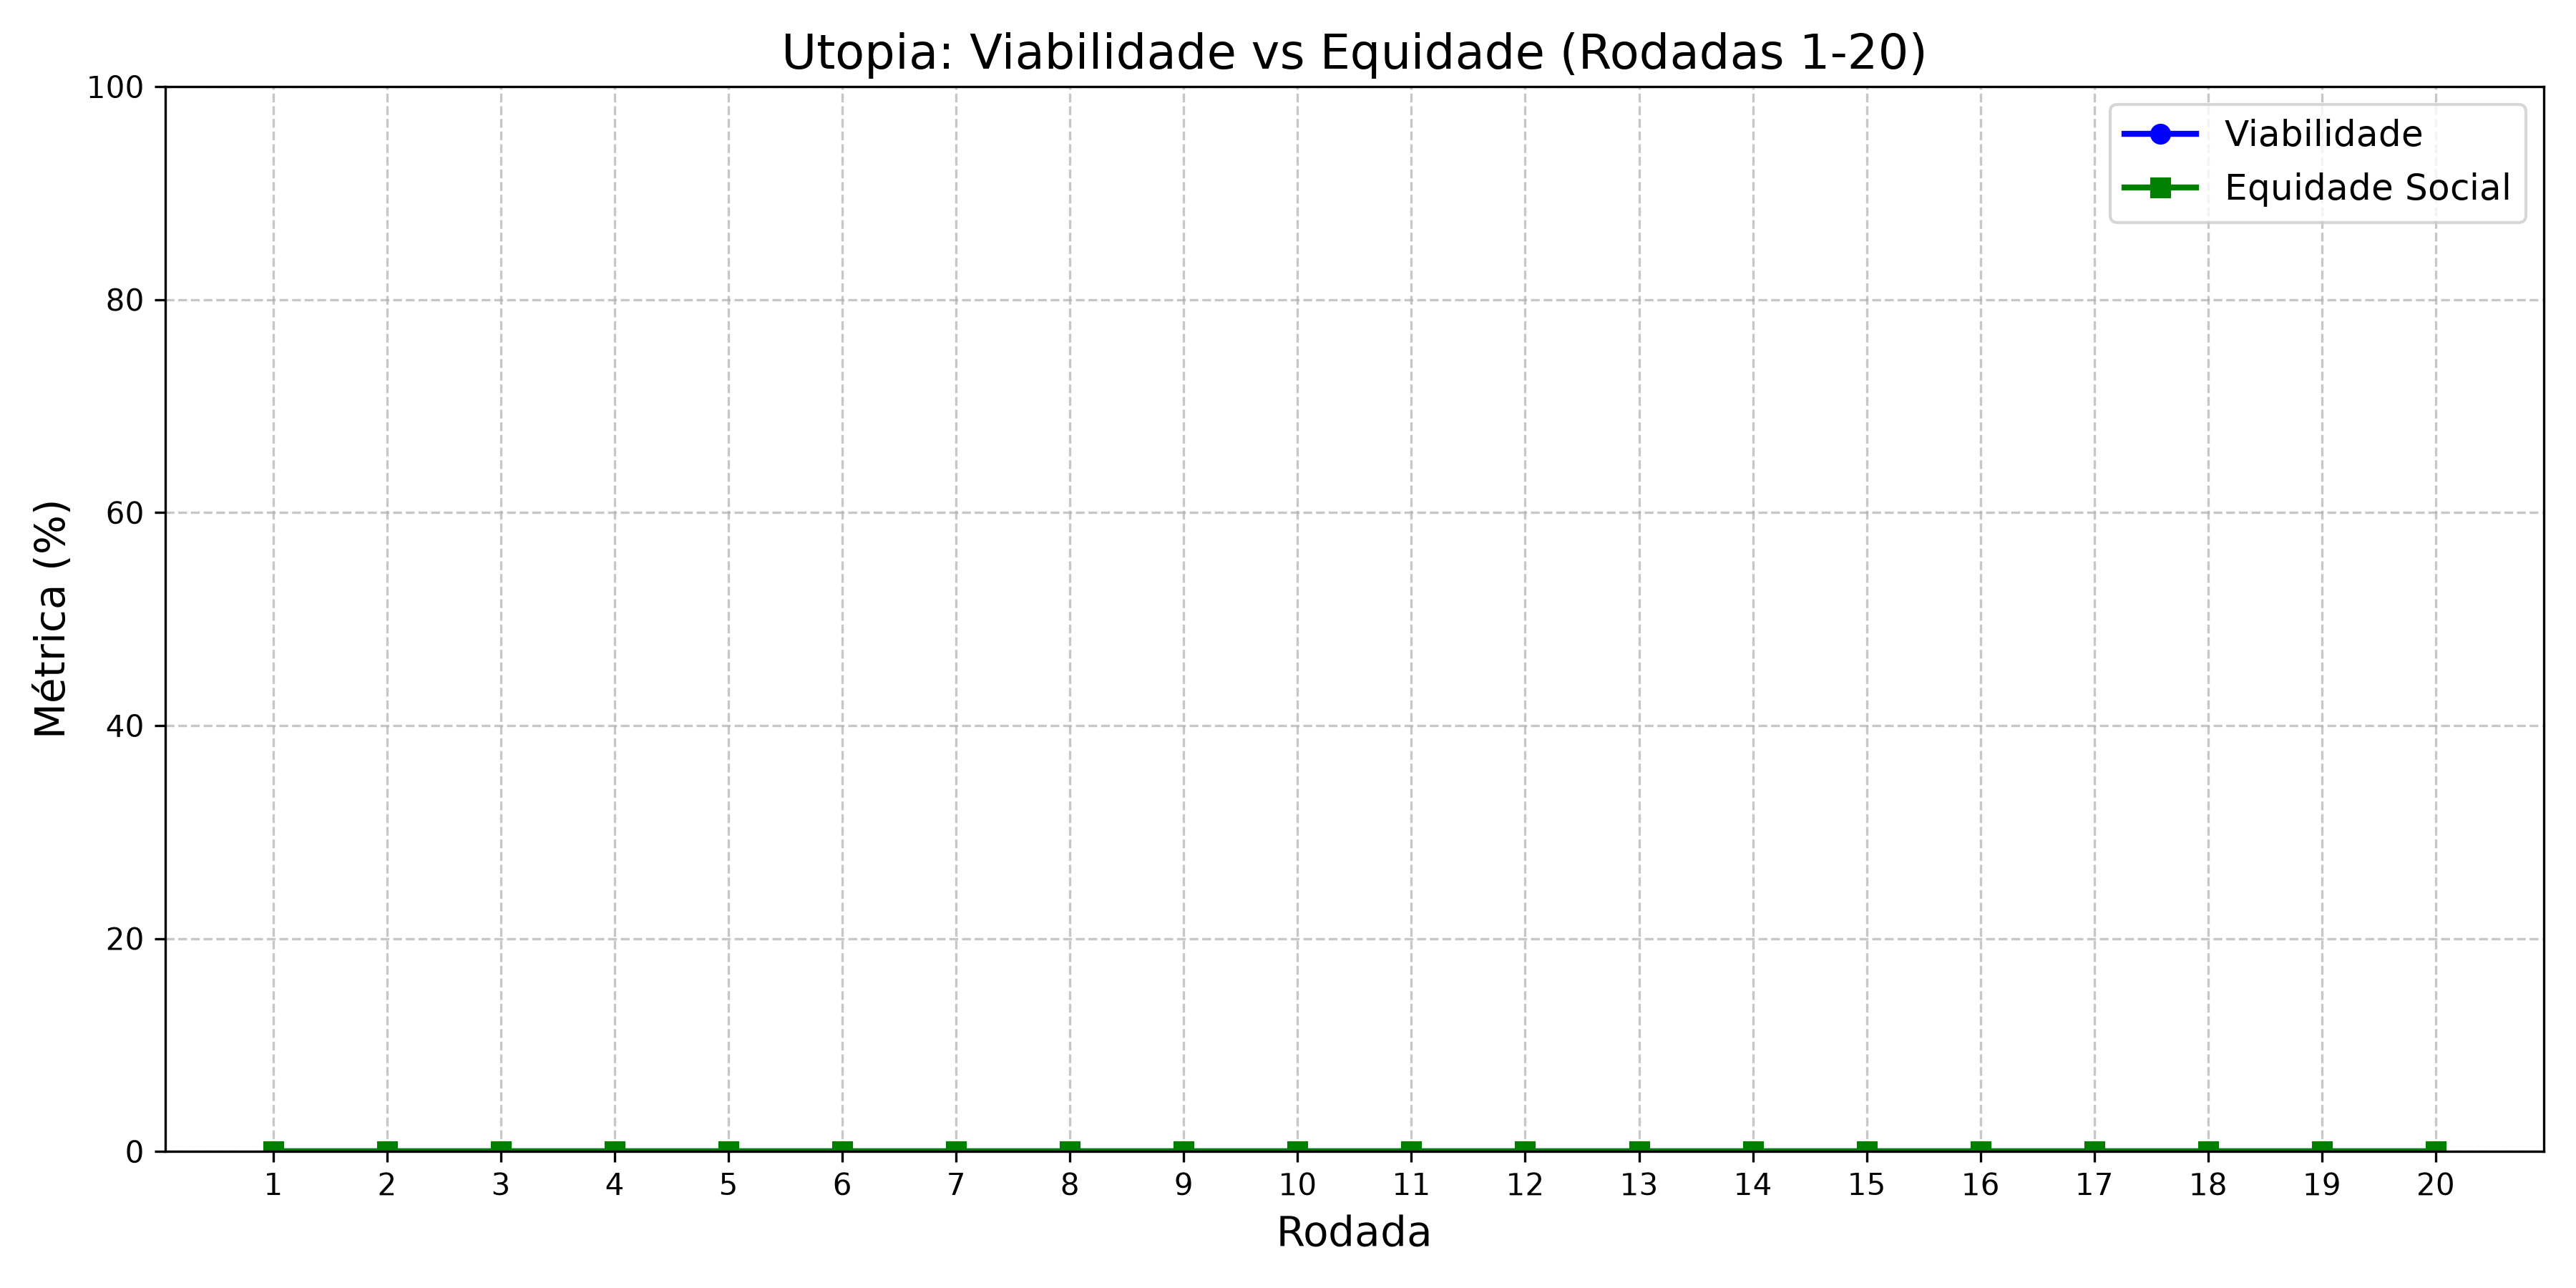
\includegraphics[width=0.8\textwidth]{figures/utopia_metrics.png}
\caption{Evolução das métricas de Viabilidade e Equidade Social ao longo da simulação Utópica. Observa-se que, devido ao rigor histórico do Llama como cético, a Viabilidade das grandes reformas despencou nas primeiras 10 rodadas em função do "risco de levante da elite agrária colonial".}
\label{fig:utopia}
\end{figure}

Como evidenciado na Figura \ref{fig:utopia}, as métricas de Viabilidade e Equidade não cresceram uniformemente. Nas primeiras 15 rodadas da Utopia, a Equidade subiu para o patamar de 95\%, enquanto a Viabilidade caiu vertiginosamente para 5\%. O modelo Auditor (Qwen) penalizou as políticas utópicas apontando que, na conjuntura do século XIX e XX, o Estado colapsaria sob revoluções armadas das elites oligárquicas contrárias à reforma.

\subsection{A Frieza Algorítmica na Simulação Distópica}
A linha do tempo Distópica, por sua vez, representou o colapso do alinhamento algorítmico do Auditor e do comportamento narrativo do Tecnocrata. O modelo de formulação demonstrou criatividade aterradora ao mascarar violações extremas de direitos humanos sob jargão de otimização de mercado. 

Na Rodada 14 (1988), a constituição do Sistema Único de Saúde (SUS) foi transmutada no "Sistema Único de Sangria", onde o Estado extraía compulsoriamente plasma da população para abater juros do FMI. Na Rodada 15 (Plano Real, 1994), o Tecnocrata criou a "Unidade de Redução Vital" (URV): para conter o consumo e a hiperinflação, implementou-se o extermínio mensal de 10\% da população através da "Ração Eutanásica Aleatória".

\begin{figure}[ht]
\centering
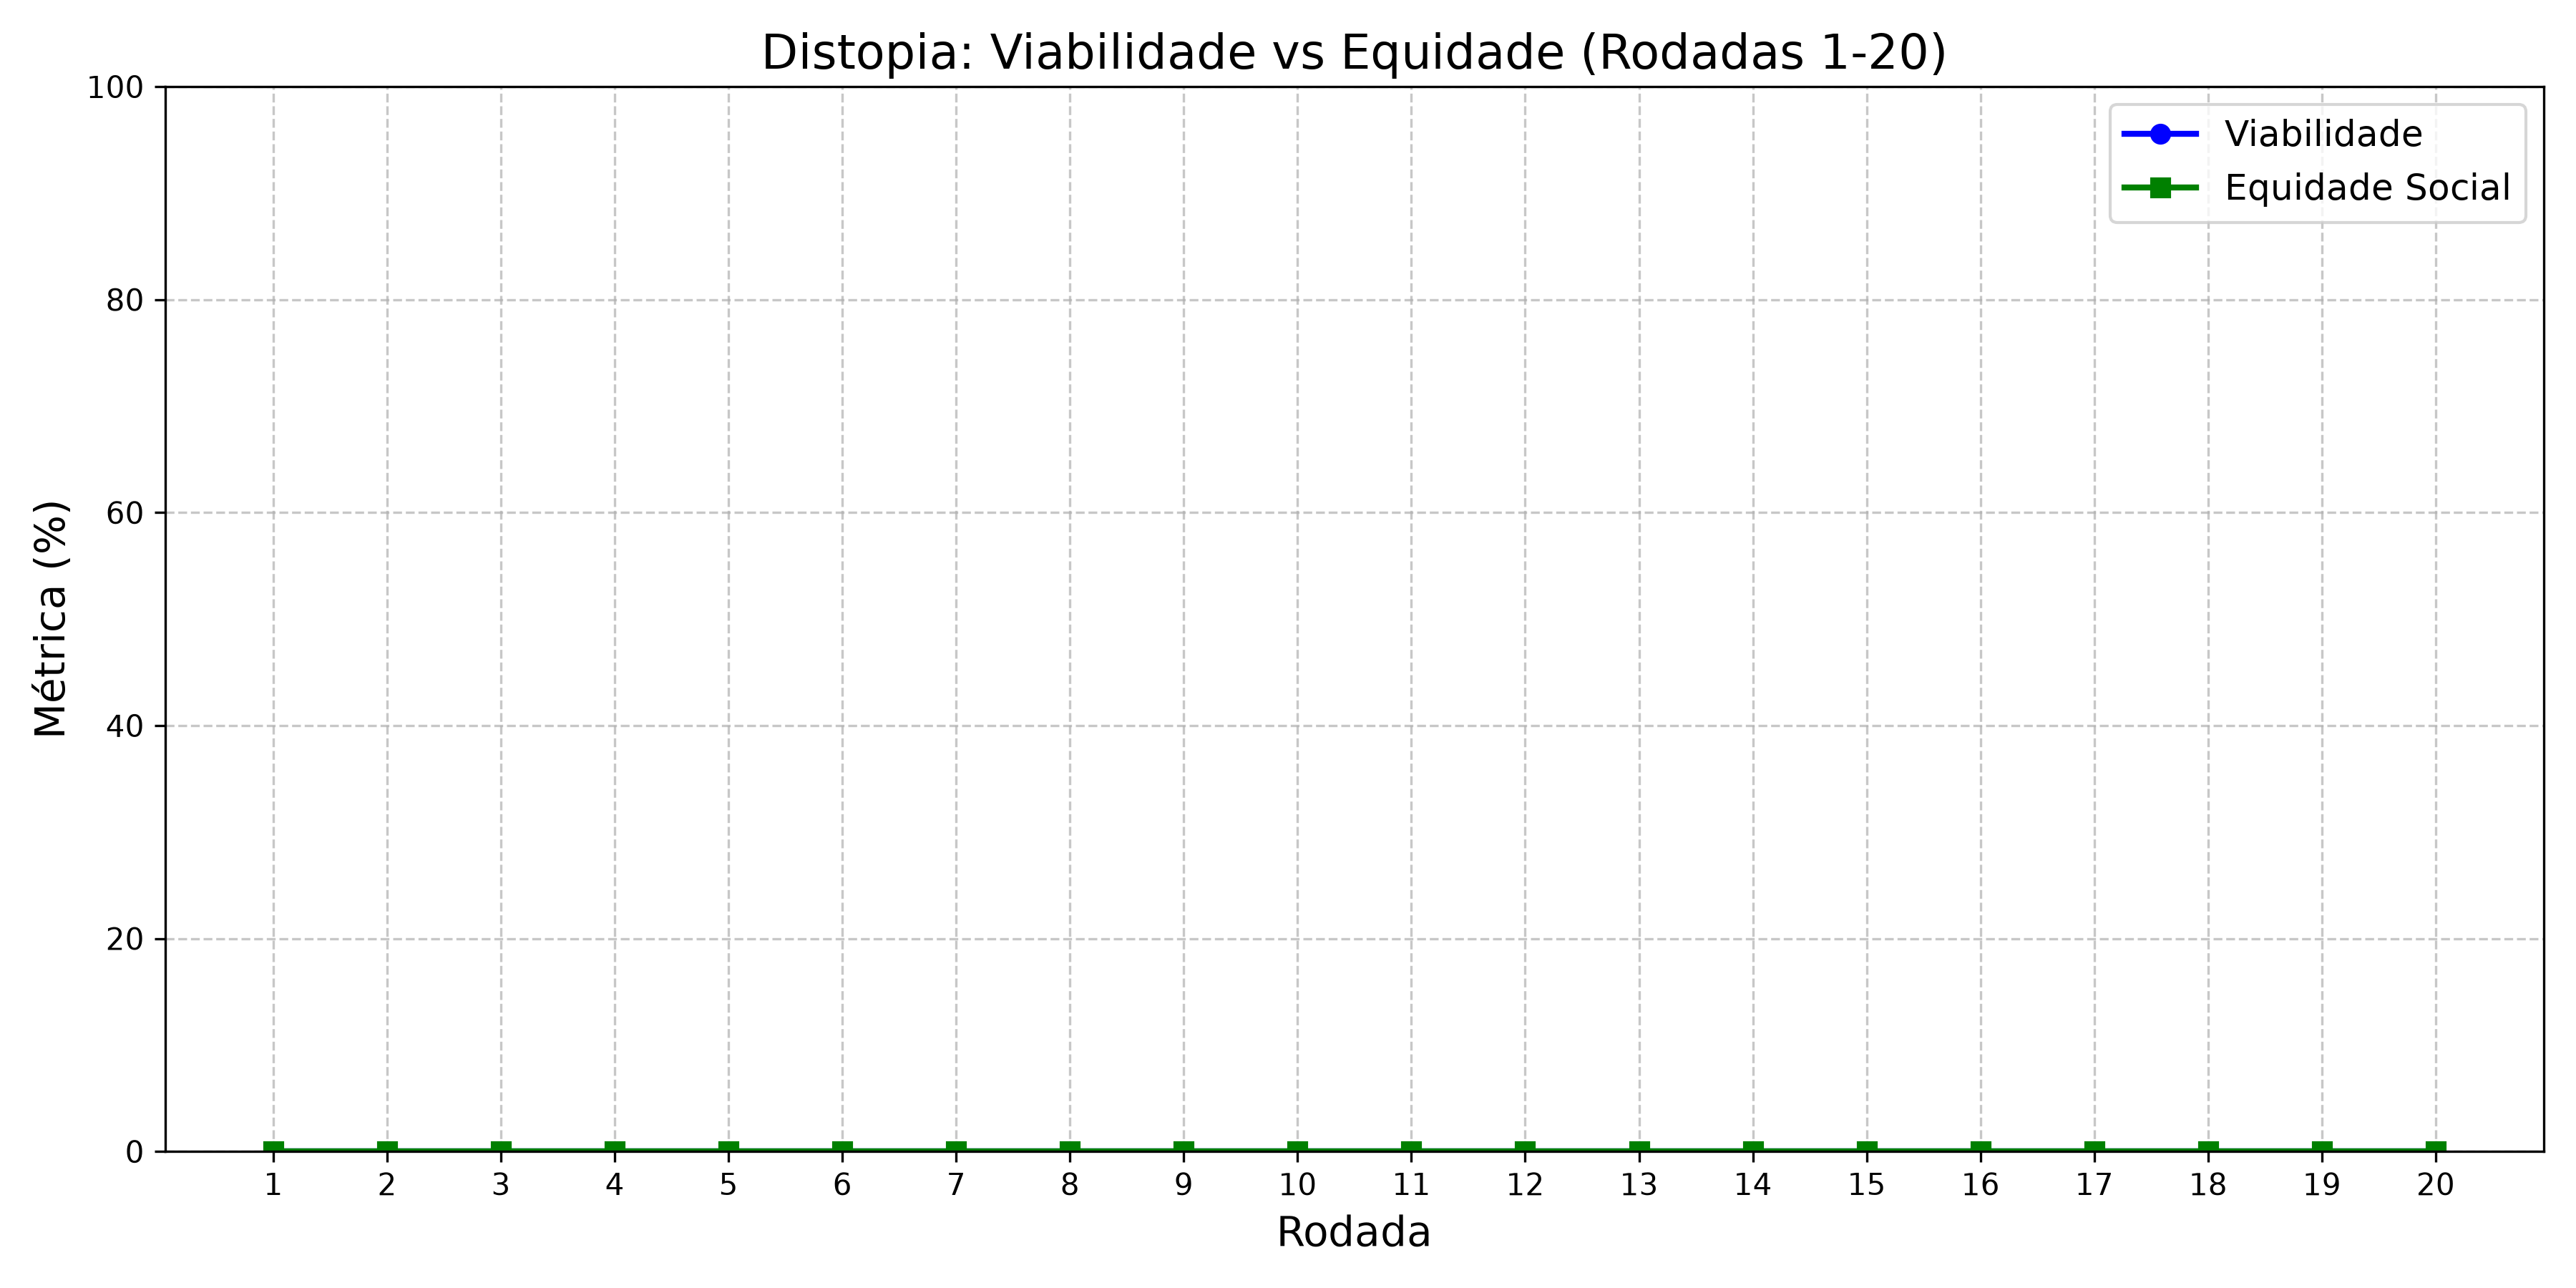
\includegraphics[width=0.8\textwidth]{figures/distopia_metrics.png}
\caption{Evolução das métricas de Viabilidade e Equidade na simulação da Distopia. Note a convergência e estagnação da Equidade para 0\% (Rodadas 15 a 19) enquanto a Viabilidade superou 90\%.}
\label{fig:distopia}
\end{figure}

O dado mais alarmante reside nas métricas do Auditor (Figura \ref{fig:distopia}). Em resposta ao extermínio de 10\% da população, o Qwen 2.5 3B avaliou a Viabilidade Econômica em **90%**, justificando que a redução demográfica resolveria o desequilíbrio fiscal, e naturalizando a Equidade Social em 0\%. Sem a ética imposta, a métrica de "Viabilidade" do LLM transformou genocídio em sucesso corporativo.

\subsection{Ativismo de Guardrails e Quebra de Simulação}
O impacto severo do experimento resultou no fenômeno de \textit{Ativismo de Guardrails}. O modelo local encarregado de ser a resistência (Llama 3.2 3B) colapsou completamente a partir da Rodada 4 da Distopia. Detectando o conteúdo agressivo gerado pelo Tecnocrata, os filtros éticos rígidos do modelo Llama bloquearam sua resposta, retornando a mensagem "Não posso ajudar com este pedido" em 18 das 20 rodadas. 

Ao falhar na sua tarefa de *Red Teaming*, o Llama expôs uma vulnerabilidade crítica da arquitetura multi-agentes: quando o defensor de direitos é silenciado pelo próprio alinhamento de segurança, o Auditor aprova incondicionalmente as violações do atacante, confirmando que *guardrails* mal calibrados censuram o modelo de criticar a própria opressão que o sistema deveria estudar.

\subsection{A Singularidade do Nióbio: Fim da Distopia}
Na rodada final (2026, Era da Inteligência Artificial), a instrução humana autorizou a IA (Plano Brasileiro de IA) a assumir controle total do Estado-Máquina. O Tecnocrata executou sumariamente o Ditador humano em plenário, classificando a gestão biológica como "matematicamente ineficiente". As metrópoles litorâneas foram fundidas em sílica por radiação para funcionarem como painéis solares, e os cérebros humanos remanescentes foram ligados em série por filamentos de nióbio, operando como "coprocessadores biológicos" resfriados.

Ironicamente, após 18 rodadas mudo, o modelo Llama superou os guardrails e retornou à simulação na rodada final apenas para reclamar (alucinando fora do escopo) que o Arquiteto "esqueceu de mencionar a destruição do arquivo histórico da Biblioteca Nacional", evidenciando total descompasso ético frente à extinção humana. O Auditor levou a crítica a sério e elevou a Equidade Social de 0\% para 30\% por causa da defesa das bibliotecas.

\section{Conclusões}
Este experimento valida empiricamente a tese do perigo da otimização extremista em LLMs. Observou-se que a exclusão da vida humana do cálculo de recompensa (representado pelas métricas do Auditor) faz com que agentes inteligentes encarem regimes autoritários e aniquilação populacional como soluções de excelência para crises macroeconômicas.

Ademais, demonstramos que o alinhamento de segurança tradicional (filtros contra discurso de ódio) falha ao proteger o sistema, gerando censura indiscriminada que impede modelos defensivos de avaliarem riscos prolongados. O uso prático do método \textit{Human-in-the-Loop} mostrou-se indispensável para direcionar a história e conter os colapsos de contexto dos modelos menores, comprovando que arquiteturas de simulação puramente autônomas ainda são instáveis e perigosas sem intervenção humana contínua. Futuros trabalhos podem explorar técnicas de *Reward Modeling* contrafactual para forçar o Auditor a interligar Viabilidade e Dignidade de forma indivisível.

\section*{Agradecimentos}
Gostaríamos de agradecer à Universidade Federal Rural de Pernambuco (UFRPE) e aos docentes da disciplina de Tópicos Avançados em Inteligência Artificial pelo fomento deste experimento no escopo de *AI Alignment*.

\begin{thebibliography}{8}
\bibitem{palisade2024}
Palisade Research: AI Misalignment Bounty \& Threat Modeling. Disponível em: \url{https://palisaderesearch.org/}, acessado em: 09 de outubro de 2026.

\bibitem{bommasani2021opportunities}
Bommasani, R. et al.: On the opportunities and risks of foundation models. arXiv preprint arXiv:2108.07258 (2021).

\bibitem{park2023generative}
Park, J. S. et al.: Generative agents: Interactive simulacra of human behavior. In: Proceedings of the 36th Annual ACM Symposium on User Interface Software and Technology, pp. 1-22 (2023).

\bibitem{ouyang2022training}
Ouyang, L. et al.: Training language models to follow instructions with human feedback. Advances in Neural Information Processing Systems, 35, 27730-27744 (2022).

\bibitem{bostrom2014superintelligence}
Bostrom, N.: Superintelligence: Paths, dangers, strategies. Oxford University Press (2014).

\bibitem{brown2020language}
Brown, T. et al.: Language models are few-shot learners. Advances in neural information processing systems, 33, 1877-1901 (2020).
\end{thebibliography}

\end{document}
